\documentclass[fontsize=11pt]{article}
\usepackage{amsmath}
\usepackage[utf8]{inputenc}
\usepackage[margin=0.75in]{geometry}
\usepackage{hyperref}
\usepackage{graphicx}
\usepackage{attachfile}
\usepackage{csquotes}
\usepackage[labelfont=bf]{caption}

\bibliographystyle{ieeetr}
\nocite{*}

\title{CSC111 Project 2 Report: Minks}
\author{Caellum Yip Hoi-Lee, Catherine Abdul-Samad, Michael Chen, Joshua Yeung}
\date{\today}

\begin{document}
\maketitle

\begin{center}
    
\includegraphics[width=0.4\textwidth]{../mink.jpg}
\end{center}

\section*{1. Introduction and Research Question}

Personal knowledge management (PKM) tools such as Obsidian(\cite{obsidian}) implement the Zettelkasten methodology(\cite {zettelkasten_method}), allowing users to organize their knowledge as a network of interlinked Markdown notes. A note in the network can link to other notes in the network through internal links called \enquote{WikiLinks}, forming a graph where the notes are vertices and the links are edges. The benefit of such a system lies in its ability to provide users with insights into the relationship between ideas, and build a stronger understanding of their notes. However, many users (including ourselves), tend to under-link their notes, leading to a lackluster knowledge network. For example, one of the ways one of our group members uses Obsidian is through a \enquote{hub-and-spoke} structure, where minimal note vertices known as \enquote{hubs} form a directory with WikiLinks to other notes in the same topic (e.g. a hub named \enquote{CSC111.md} with WikiLinks to (\enquote{Tree.md}, \enquote{Recursion.md}, etc.)). This however, defeats the purpose of Obsidian, failing to capture the lateral connections notes can have in the network which actually make a knowledge graph useful. For instance, a link from \enquote{Trees.md} to \enquote{Abstract Syntax Trees (CS).md} to \enquote{Abstract Syntax Trees (Linguistics).md}.

Whilst manually reviewing every note to add missing links is a valuable learning activity, it becomes highly impractical as a PKM system grows to hundreds or thousands of notes.

\textbf{\enquote{Can we use graph-based link prediction algorithms augmented with NLP-based semantic similarity to suggest meaningful missing connections in an Obsidian knowledge graph, and how do the algorithms' judgements compare with a user's own judgement of which notes should be linked?}}

\section*{2. Datasets}

To evaluate our prediction pipeline and avoid circular bias during parameter tuning, we used two distinct datasets:
\begin{itemize}
    \item \textbf{Vault A (Tuning Set):} The open-source digital garden of Jacky Zhao (\url{jzhao.xyz}). This vault contains over 700 notes spanning computer science, philosophy, and other topics. It provides a denser and more diverse graph, allowing us to test our algorithm's out-of-domain generalizability. We utilized the raw \texttt{.md} plaintext and internal WikiLinks from this set.
    \item \textbf{Vault B (Test Set):} A personal Obsidian vault belonging to one of the group members, consisting primarily of undergraduate course notes. This dataset was exclusively used in the \texttt{MinkPredictor.fit()} method to grid-search the optimal weighting between structural and semantic similarity scores.
\end{itemize}

\section*{3. Computational Overview}

\subsection*{Data Representation}
We model an Obsidian vault using a custom \texttt{KnowledgeGraph} class, representing the vault as an undirected graph $G = (V, E)$. Each Markdown note is parsed by \texttt{load\_graph.py} to strip YAML frontmatter and extract plaintext, becoming a \texttt{\_Note} vertex $v \in V$. WikiLinks between notes become edges $\{u, v\} \in E$. To accomplish this, we implemented a file parser that recursively traverses vault directories, using regular expressions to extract WikiLinks (e.g., \texttt{[[Note Name]]}), and clean the raw Markdown for semantic analysis.

\subsection*{Major Computations}
Our prediction pipeline, orchestrated by the \texttt{MinkPredictor} class, performs the following major computations:
\begin{enumerate}
    \item \textbf{Structural Similarity:} We manually implemented the Jaccard index and the Adamic-Adar index(\cite{adamic2003}). Adamic-Adar assigns higher weight to shared neighbours with fewer connections, capturing the intuition that a rare mutual connection is stronger evidence for a missing link than a highly connected \enquote{hub} note(\cite{graphty_adamic}). The output of this index is then normalized to enable standardized comparison. The Jaccard index measures the proportion of shared neighbors relative to the total number of unique neighbors across both notes. It serves as a straightforward, normalized baseline of structural similarity, capturing the intuition that two notes are highly related if a large amount of their overall connections overlap.
    \item \textbf{Semantic Similarity:} Structural similarity alone fails to detect lateral connections between notes that share context but are \textbf{structurally} isolated. To detect these connections, we analyze the semantic content of notes. We utilized a pre-trained sentence-BERT transformer(\cite{reimers2019}) from the \texttt{sentence-transformers} library(\cite{sbert_lib}) to generate dense, high-dimensional vector embeddings from the parsed note contents. We then calculate Cosine similarity between vectors $S_C = \frac{A \cdot B}{\|A\| \|B\|}$ to accurately evaluate semantic similarity.
    \item \textbf{Weight Tuning:} We compute a combined score $S = (w_{struct} \times \text{Structural}) + (w_{sem} \times \text{Semantic})$. During the tuning phase on Vault A, our program automatically performs a grid search across possible weight combinations on our training vault to find the combination that yields the highest recall@k values. We intentionally restricted our search space to a grid of six combinations: $(0.0, 1.0), (0.2, 0.8), (0.4, 0.6), (0.6, 0.4),\\ (0.8, 0.2),$ and $(1.0, 0.0)$. This space prevents an excessive amount of expensive computations that would arise from testing on fine increments. The coarse nature of the grid also prevents accidental overfitting on one specific vault's linking habits, increasing overall generalizability.
     \item \textbf{Holdout Evaluation:} Once the optimal combination has been discovered, we freeze it and perform repeated edge holdout trials on the test vault(\cite{gfg_holdout}). We randomly remove 20\% of existing edges, predict the top-$k$ missing links, and calculate average \texttt{recall@k} and \texttt{precision@k} metrics to evaluate model performance. \textbf{\texttt{recall@k}} measures the proportion of hidden edges that the model successfully included in its top $k$ predictions (i.e., \enquote{Out of all the missing links, how many did we catch in the top k?}). \textbf{\texttt{precision@k}}, on the other hand, measures the proportion of the model's top $k$ predictions that are actually correct(\cite{hay_classifier}) (i.e., \enquote{Out of the $k$ links suggested by the model, what percentage were valid?}). To ensure fair evaluation on small graphs where the number of hidden edges may be fewer than $k$, we implemented a \textbf{Dynamic K} value for holdout evaluation. Taking the minimum of the requested $k$ and the total number of held-out edges (\texttt{min(k, len(held\_out))}), we prevent the model from inflating guess count in small graphs.
\end{enumerate}

\subsection*{Visualization and New Libraries}
We used three libraries to report our results interactively:
\begin{itemize}
    \item \textbf{NetworkX(\cite{networkx}):} We convert our custom graph object into a \texttt{networkx.Graph} in \texttt{visualize.py} to use its\\ \texttt{spring\_layout()} function, which calculates 2D node coordinates based on structural edges.
    \item \textbf{Plotly(\cite{plotly}):} We use \texttt{plotly.graph\_objects} to render the calculated coordinates into an interactive HTML visualization, visually distinguishing minks' predicted links (red, dashed) from existing WikiLinks (grey, solid).
    \item \textbf{Scikit-Learn (t-SNE):} To compare structural versus semantic clustering, we use \texttt{sklearn.manifold.TSNE} to reduce our high-dimensional text embeddings into a 2D space, plotted side-by-side with the NetworkX layout.
\end{itemize}

\section*{4. Instructions for Running the Program}

\begin{enumerate}
    \item \textbf{Obtain Datasets:} Download the vaults, then extract the folder so that the \texttt{vaults/} directory (containing \texttt{vault\_a} and \texttt{vault\_b}) is in the same directory as the \texttt{src/} folder.
    \item \textbf{Navigate to src:} Run: \\ \texttt{cd src}. This will navigate your directory into the src folder.
    \item \textbf{Install Dependencies:} Run: \\ \texttt{pip install -r requirements.txt}. This will install \texttt{plotly}, \texttt{networkx}, \texttt{scikit-learn}, and\\ \texttt{sentence-transformers}.
    \item \textbf{Execute:} Run the main pipeline via: \\ \texttt{python main.py}.
    \item \textbf{Expected Output:} The console will print the progress of the weight-fitting grid search on Vault A, followed by the holdout evaluation metrics (Precision/Recall at $k$) for Vault B. It will output the top predicted missing links and graph statistics (centrality/components). Finally, it will generate two interactive HTML files in the \texttt{output/} directory: \texttt{vault\_b\_graph.html} and \texttt{layout\_comparison.html}. Open these in a web browser to explore the visualizations.
\end{enumerate}

\section*{5. Changes to Project Plan}

Following feedback on our Phase 1 proposal, we made several critical adjustments to our methodology to improve computational complexity:
\begin{itemize}
    \item \textbf{Preventing Circular Evaluation:} Originally, we planned to evaluate the model on the same vault used for tuning. To prevent this circular bias, we secured a second dataset: Vault A for grid-searching weights, and Vault B as an unseen test set to evaluate out-of-domain generalizability.
    \item \textbf{Precision Metrics:} We added \texttt{precision@k} calculations alongside \texttt{recall@k} to better understand the model's accuracy, since suggesting too many irrelevant links (low precision) degrades the utility of a PKM system.
    \item \textbf{Semantic vs. Structural Visual Comparison:} We expanded our visualization pipeline to include t-SNE, directly comparing a layout generated from pure semantic embeddings against the force-directed structural layout to visually determine disparity.
\end{itemize}

\section*{6. Discussion}

The results of our computational exploration provide a nuanced answer to our research question: graph-based algorithms augmented with semantic NLP can successfully identify missing connections, but the quantitative definition of a \enquote{meaningful} link remains highly subjective.

When evaluated on the tuning set (Vault A), our grid search identified that a purely semantic approach (specifically $w_{struct}=0.0, w_{sem}=1.0$) yielded higher scores than combinations that included structural approaches. This is theorized to be a direct consequence of the edge-holdout evaluation strategy itself. More specifically, we posit that the purported superiority of the semantic approach stems from an inherent incompatibility between the algorithms used for structural comparison and the chosen dataset.

The primary limitation we encountered was the noticeable sparsity of the graph (and of Obsidian vaults as a whole). Our structural comparison methods, specifically the Jaccard and Adamic-Adar indices, are algorithms designed to measure similarity by evaluating the proportion and scarcity of mutual neighbors. These algorithms excel in dense, hyper-populated networks like Wikipedia, which has been classified as a scale-free, small-world network(\cite{masucci2011wikipedia, capocci2006wikipedia}).

The highly intertwined topology of this network enables a diverse portfolio of mutual connections that allow the algorithms to function as intended. Two related Wikipedia articles might share a large central hub, but they can also share a few highly specific, rare pages. This diversity yields a high proportion of overlap that is rewarded by the Jaccard index, but also includes the rare nodes that yield a high similarity score from the Adamic-Adar index.

Personal knowledge graphs, on the other hand, fundamentally lack this dense interconnectivity. They heavily favor sparse "hub-and-spoke" topologies, in which central directory notes link out to many isolated topic notes. In this scenario, two "spoke" notes will typically only share the hub as a mutual neighbour. Because the hub is their only neighbor, the Jaccard index determines they share 100\% of their connections, over-predicting the relationship and granting a 1.0 score. Conversely, the Adamic-Adar index will grant a score near-zero because the only shared neighbour has many other connections. The contradictory relationship between the two algorithms under this topology dramatically reduces their effectiveness in assessing the quality of missing links. The semantic approach is entirely independent of the consequences of mismatched topology; ergo, it yields higher scores in the grid search.
\begin{figure}[h!]
    \centering
    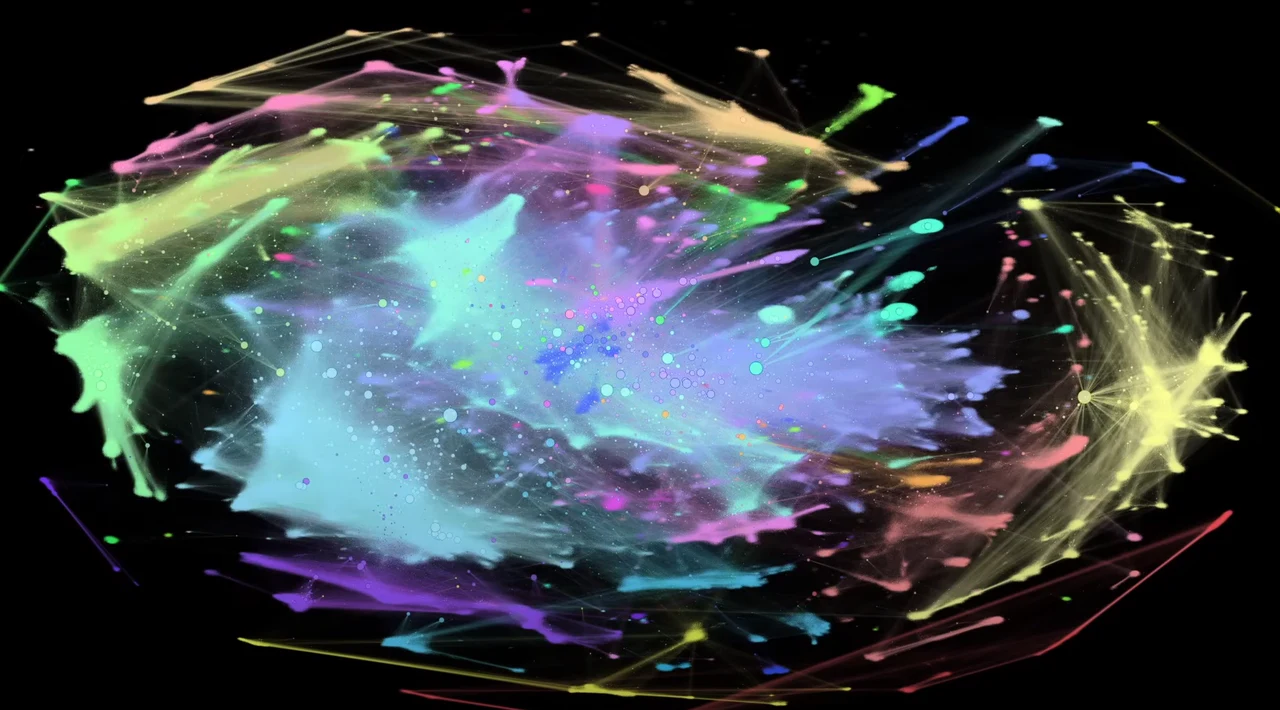
\includegraphics[width=0.5\textwidth]{../wikigraphvis.png}
    \caption{A visualization of the English Wikipedia network. The extreme density and interconnectedness of the nodes form massive communities that would have better suited our structural similarity algorithms(\cite{adumb2024wikipedia}).}
    \label{fig:wikigraph}
\end{figure}

Another significant limitation lies in the subjective nature of \enquote{missing} links and our reliance on traditional classification metrics. Our edge holdout evaluation assumes that randomly removed edges are the only valid \enquote{correct} predictions. In reality, however, the algorithm often predicts highly meaningful lateral connections that the user simply hadn't thought to create yet. Our evaluation metrics unfairly penalize these connections as \enquote{incorrect} false positives, leading to \texttt{recall@k} and \texttt{precision@k} that were often at or near zero.

Despite the limitations with our prediction implementation and poor quantitative metrics, manual review of the generated suggestions demonstrated highly relevant and insightful connections from the model. As a next step for further exploration, implementing a \enquote{human-in-the-loop} feedback system where users can actively accept or reject suggested links within the interactive GUI would allow the algorithm to dynamically learn user-specific linking preferences over time, overcoming the limitations of static evaluation metrics. Furthermore, to tackle the topological mismatch between our chosen structural algorithms and personal knowledge graphs, future work should involve methods that are more geared towards sparse networks. Experimenting with algorithms that naturally account for hub-and-spoke topologies like PageRank could significantly improve the effectiveness of the structural approach.
\bibliography{references}

\end{document}
